\subsection{UC26 - Modifica informazioni utente}\label{usecase:26}
\begin{figure}[H]
\centering
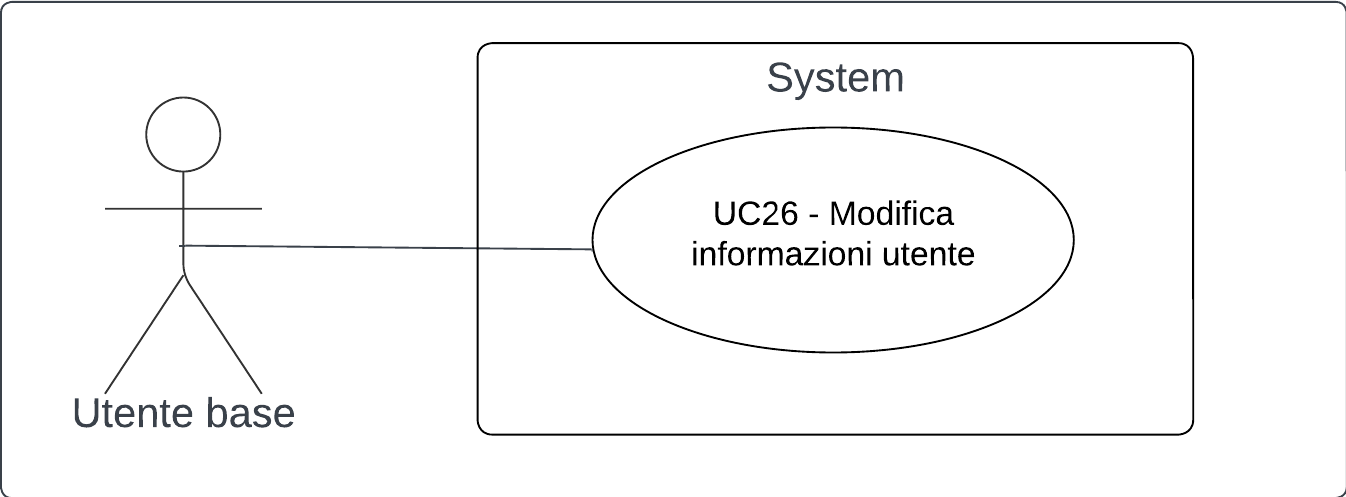
\includegraphics[width=0.75\linewidth]{ucd/UCD26}
\caption{Modifica informazioni utente}
\end{figure}
\textbf{Attori}:
\begin{itemize}
    \item Utente base.
\end{itemize}
\textbf{Precondizioni}:
\begin{itemize}
    \item L'utente base è connesso al $\textit{sistema}_G$.
\end{itemize}
\textbf{Postcondizioni}:
\begin{itemize}
    \item L'utente ha modificato le informazioni sul suo profilo.
\end{itemize}
\textbf{Scenario principale}:
\begin{enumerate}
    \item L'utente modifica :
    \begin{itemize}
        \item Il suo nome;
        \item Il suo cognome;
        \item La email;
        \item La sua password.
    \end{itemize}
\end{enumerate}
\textbf{Scenari alternativi}:
\begin{enumerate}
    \item Nel caso in cui l'email sia già presente all'interno del $\textit{sistema}_G$ oppure non sia valida, l'utente viene notificato attraverso un messaggio;
    \item Viene data la possibilità all'utente di scegliere un'altra email valida.
\end{enumerate}
\newpage